\chapter{Training \& Testing of the
Classifier}
\label{Chapter 4}
Recall from the last chapter that Convolutional Neural Networks (CNNs) are used
in the training of a model for a classifier. Classification is the process
of putting a tag on an image from a set of class labels. This chapter is about the
training of classifier for a dataset of 10000 images with 2000 images of each class.
The step by step process of training a classifier is explained in detail in this chapter. Results obtained from the testing of the classifier by varying certain parameters are recorded and attached
in the latter part of the chapter.
\section{Formation of Dataset}
In deep learning techniques for Classification of images, we have
an example of images which are input to to the system to get a
label from the given classes. This set of images is called dataset.
The dataset is divided into training and dataset by a specific ratio.


In this project we have five different classes of vehciles i.e. Bus, Car, Truck, Motorcycle
and Hiace. There are a total of 10000 images with 2000 images of each 
class. These images are downloaded from Google search results and from already available
datasets and from websites providing licensed free images like Flickr. APIs are available which
can be used along with a simple Python script to download a lot of images.
Using matplotlib in python, we can plot some of the images with the output as
shown in listing \ref{listing:4.1} and plot is attached in figure
\ref{fig:4.1}.
\begin{listing}[H]
\begin{minted}[bgcolor=bg,
    frame = lines,
    framesep = 2mm]{python}
import matplotlib.pyplot as plt
from matplotlib.image import imread  
path  = './images/'
for i in range(9):
    plt.subplot(330+1+i)
    filename = path + 'image_'+ str(i) + '.jpg'
    image = imread(filename)
    plt.imshow(image)    
    plt.show()
\end{minted}
\caption{Python script to plot some images from each class}
\label{listing:4.1}
\end{listing}

\begin{figure}[H]
    \centering
    \captionsetup{justification = centering}
    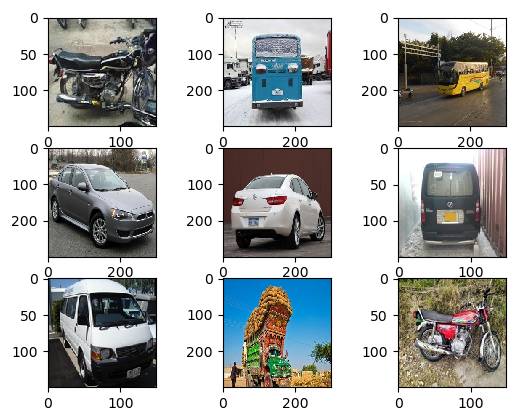
\includegraphics[scale = 0.8]{CHAPTERS/Chapter-4/Images/4.1.png}
    \caption{Plot of some images from each class} 
    \label{fig:4.1}
  \end{figure}

\subsection{Data Augmentation}
Increasing the size of dataset makes the deep learning model to learn and classify images more accurately. This problem of lack of sufficient data can be solved using technique of data augmentation which is used to increase the size of available set of images.
Data augmentation is the process of applying techniques like shifting, flipping, rotating and varying the brightness etc on images to introduce variations among them.
This technique is used within the code using Keras.
\section{Setting of Workspace for the Project}
There are a lot of images to be processed. To process images, high end GPU is
needed. Due to unavailability of an Nvidia GPU in the system, we used Google Colab.
It is an online platform having high end GPUs free provided by Google for training
up to 12 hours. Enabling a gpu in the notebook settings can accelerate the process of
training.
\section{Working of Code}
Keras is one of the leading high level API for neural networks. It contains
many modules such as layers, cost functions, activation functions, initialization
schemes and regularization schemes. This project uses Keras for training purposes.
\subsection{Conversion of Images and Labels to Numpy Arrays}
After importing all the necessary packages, we are all set to pre process our data.
Recall to chapter 2, where we studied the basics of an image. In Keras image has two
representations i.e. (width, height, color\_channels) and (color\_channels, width, height).
First approach is called as channels first approach and the latter is called as
channels last approach. We will use the channels last approach.
First step is to read the images from the folder (uploaded to Colab),
Labels are assigned to classes from 0 to 4. Keras load\_img() loads image from the folder given
target size. Target size for this project is chosen as 128 by 128. This means width and height,
both are 128. Color channels fro RGB images are 3. Images are then converted to numpy arrays using
Keras img\_to\_array() method. Labels are stored as 0, 1, 2, 3, 4 based on the class of image (as data is renamed).
A section of code for this implementation is shown in listing \ref{listing:4.2}.

\begin{listing}[H]
    \begin{minted}[bgcolor=bg,
        frame = lines,
        framesep = 2mm]{python}
folder = '/content/Input_data/'
photos = np.zeros((num_of_images,img_rows,img_cols,color_channels))
labels = np.zeros(num_of_images)
i = 0
# enumerate files in the directory
for file in os.listdir(folder):
# determine class
    if file.startswith('bus'):
        output = 0
    elif file.startswith('car'):
        output = 1
    elif file.startswith('bike'):
        output = 2
    elif file.startswith('hiace'):
        output = 3
    else:
        output = 4
    # load image
    img = load_img(folder + file, target_size=(img_rows,img_cols))
    # convert to numpy array
    img = img_to_array(img)
    # store
    images[i] = img
    labels[i] = output
    i = i+1
\end{minted}
\caption{Conversion of Images to Numpy arrays}
\label{listing:4.2}
\end{listing}
The images array has a pattern (num\_of\_images, rows, cols, color\_channels). It
means that it has a shape (10000, 128, 128, 3). This is a 4D tensor. There are 10000
images with each image having 128, $128\times 3$ matrices i.e. each $128\times 3$ matrix has
128 rows with each row containing 3 columns with information of 3 colors.
The labels array is a 1D tensor with 10000 \% labels.
\subsection{Train-Test Division}
We have to divide the data into two parts, train and test. The training data
is used to for training purposes and when the model is trained then it is
used to test the model using the test images and test labels. We used a ratio of 75\% and
25\% for train and test respectively. The package used for this purpose is the
Scikit-learn train\_test\_split. Listing \ref{listing:4.3} shows splitting of
data into train and test.

\begin{listing}[H]
    \begin{minted}[bgcolor=bg,
        frame = lines,
        framesep = 2mm]{python}
train_images, test_images, train_labels, test_labels = 
train_test_split(images, labels, test_size = 0.25, random_state = 42)
\end{minted}
\caption{Train-test split}
\label{listing:4.3}
\end{listing}
There is another technique for splitting of data. We make two directories
train and test and randomly divide the images into these directories and then
convert them into numpy array. Here we have first converted the images
into arrays, split them into train and test and then we can save them back into
directories by converting them into images from array using PIL from\_array
function.

\subsection{Mean Correction}
After converting to float 32 and normalizing by 255, we have to subtract mean pixel.
Listing \ref{listing:4.4} illustrates the mean correction.

\begin{listing}[H]
    \begin{minted}[bgcolor=bg,
        frame = lines,
        framesep = 2mm]{python}
if subtract_pixel_mean:
x_train_mean = np.mean(train_images, axis=0)
train_images -= x_train_mean
test_images -= x_train_mean
train_labels = to_categorical(train_labels,num_classes)
test_labels = to_categorical(test_labels,num_classes)
    \end{minted}
    \caption{Mean correction}
\label{listing:4.4}
\end{listing}
\noindent The last two lines are categorical labeling for using labels fit for Keras.
\subsection{Defining the Model}
Recall from chapter \ref{Chapter 3}, a CNN model consists of various layers including
conv2D, Activation, MaxPoooling2D, Flatten and Dense layer. Listing \ref{listing:4.5}
defines the training Model.

\begin{listing}[H]
    \begin{minted}[bgcolor=bg,
        frame = lines,
        framesep = 2mm]{python}
#Model
model = Sequential()
model.add(Conv2D(32, (3, 3), padding='same',
                         input_shape=train_images.shape[1:]))
model.add(Activation('relu'))
model.add(Conv2D(32, (3, 3)))
model.add(Activation('relu'))
model.add(MaxPooling2D(pool_size=(2, 2)))
model.add(Dropout(0.25))   
model.add(Conv2D(64, (3, 3), padding='same'))
model.add(Activation('relu'))
model.add(MaxPooling2D(pool_size=(2, 2)))
model.add(Dropout(0.25))      
model.add(Flatten())     
model.add(Dense(64))
model.add(Activation('relu'))
model.add(Dropout(0.5))      
model.add(Dense(num_classes))
model.add(Activation('softmax'))      
model.compile(loss='categorical_crossentropy',
                      optimizer='adam',
                      metrics=['accuracy'])
    \end{minted}
    \caption{Defining the Model}
\label{listing:4.5}
\end{listing}
Last three lines defines the compilation process of the Model. 
For more than two classes, loss is categorical\_crossentropy. For two
classes it is binary\_crossentropy. There are many optimizers in Keras i.e.
SGD, Adam, RMSprop, Adamax etc. Here we have used Adam. Metrics calculates how
often prediction equals labels.
\subsection{Fitting the Model}
Here the process of training starts. We have two functions used in Keras. One
is model.fit and other is model.fit\_generator. As we discussed in section 4.1.1
about data augmentation. Here we have implemented data augmentation using a true false
logic. We have also defined a validation set. Validation data tells us about the
behavior of the model to an unseen data.

The number of times a model goes through the data is termed as `epochs'.
We have to determine the specific number of epochs for which the training process has to
run. If we run the process above that number, the training accuracy will
increase. But when we test that model with the test data, the accuracy of the model
will be lower than the training accuracy. This process is called `\textit{overfitting}'.
We have to avoid the overfitting. We use validation data which shows us the validation accuracy
and loss after each epoch. Listing \ref{listing:4.6} shows the code for training process.
\begin{listing}[H]
    \begin{minted}[bgcolor=bg,
        frame = lines,
        framesep = 2mm]{python}
if subtract_pixel_mean:
x_train_mean = np.mean(train_images, axis=0)
train_images -= x_train_mean
test_images -= x_train_mean
train_labels = to_categorical(train_labels,num_classes)
test_labels = to_categorical(test_labels,num_classes)
    \end{minted}
    \caption{Mean correction}
\label{listing:4.4}
\end{listing}
\noindent The last two lines are categorical labeling for using labels fit for Keras.
\subsection{Defining the Model}
Recall from chapter \ref{Chapter 3}, a CNN model consists of various layers including
conv2D, Activation, MaxPoooling2D, Flatten and Dense layer. Listing \ref{listing:4.5}
defines the training Model.

\begin{listing}[H]
    \begin{minted}[bgcolor=bg,
        frame = lines,
        framesep = 2mm]{python}
if not data_augmentation:
    print('Not using data augmentation.')
    history = model.fit(train_images, train_labels, validation_data=(test_images,
    test_labels), batch_size = batch_size, epochs = n_epochs)
else:
    datagen = ImageDataGenerator(
        featurewise_center=False,  # set input mean to 0 over the dataset
        samplewise_center=False,  # set each sample mean to 0
        featurewise_std_normalization=False,  # divide inputs by std of the dataset
        samplewise_std_normalization=False,  # divide each input by its std
        zca_whitening=False,  # apply ZCA whitening
        zca_epsilon=1e-06,  # epsilon for ZCA whitening
        rotation_range=0,  # randomly rotate images in the range (degrees, 0 to 180)
        # randomly shift images horizontally (fraction of total width)
        width_shift_range=0.1,
        # randomly shift images vertically (fraction of total height)
        height_shift_range=0.1,
        shear_range=0.,  # set range for random shear
        zoom_range=0.,  # set range for random zoom
        channel_shift_range=0.,  # set range for random channel shifts
        # set mode for filling points outside the input boundaries
        fill_mode='nearest',
        cval=0.,  # value used for fill_mode = "constant"
        horizontal_flip=True,  # randomly flip images
        vertical_flip=False,  # randomly flip images
        # set rescaling factor (applied before any other transformation)
        rescale=None,
        # set function that will be applied on each input
        preprocessing_function=None,
        # image data format, either "channels_first" or "channels_last"
        data_format=None,
        # fraction of images reserved for validation (strictly between 0 and 1)
        validation_split=0.0)
        datagen.fit(train_images)
        history = model.fit_generator(datagen.flow(train_images, train_labels,
        batch_size = batch_size),validation_data=(test_images, test_labels),
        epochs = n_epochs)  
    \end{minted}
    \caption{Training the Model}
\label{listing:4.6}
\end{listing}